\documentclass{standalone}

\usepackage{ tikz }

\begin{document}
    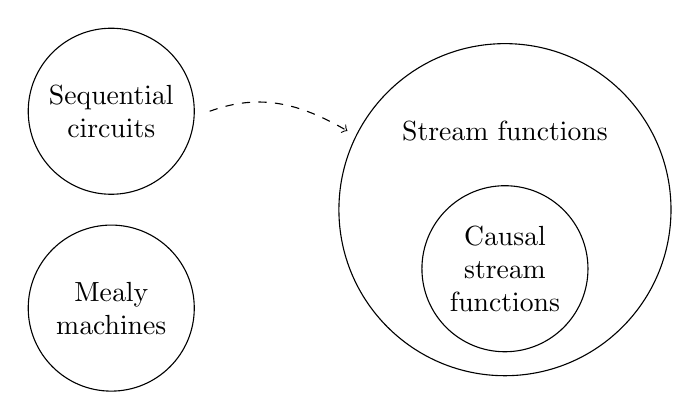
\begin{tikzpicture}
        \draw (0,1.25) circle (30pt);
        \node [align=center] at (0,1.25) {Sequential \\ circuits};
        \coordinate (SC1) at (1.25,1.25); 

        \draw (0,-1.25) circle (30pt);
        \node [align=center] at (0,-1.25) {Mealy \\ machines};

        \draw (5,0) circle (60pt);
        \node [align=center] at (5,1) {Stream functions};
        \coordinate (SF1) at (3,1);
        \draw (5,-0.75) circle (30pt);
        \node [align=center] at (5,-0.75) {Causal \\ stream \\ functions};

        \draw [->, dashed] (SC1) to[out=20,in=150] (SF1);
    \end{tikzpicture}
\end{document}